\documentclass[12pt, a4paper]{article}
\usepackage[francais]{babel}
\usepackage{caption}
\usepackage{graphicx}
\usepackage[T1]{fontenc}
\usepackage{listings}
\usepackage{geometry}
\usepackage{minted}
\usepackage{array,multirow,makecell}
\usepackage{float}
\usepackage[colorlinks=true,linkcolor=black,anchorcolor=black,citecolor=black,filecolor=black,menucolor=black,runcolor=black,urlcolor=black]{hyperref}
\setcellgapes{1pt}
\makegapedcells
\usepackage{fancyhdr}
\pagestyle{fancy}
\lhead{}
\rhead{}
\chead{}
\rfoot{\thepage}
\lfoot{Baumgaertner - Rehm - Doghmane}
\cfoot{}
\renewcommand{\footrulewidth}{0.4pt}
\renewcommand{\headrulewidth}{0.4pt}
\renewcommand{\listingscaption}{Code}
\renewcommand{\listoflistingscaption}{Table des codes}

% \usepackage{mathpazo} --> Police à utiliser lors de rapports plus sérieux

\begin{document}
\begin{titlepage}
	\newcommand{\HRule}{\rule{\linewidth}{0.5mm}} 
	\center 
	\textsc{\LARGE iut de colmar}\\[4.5cm] 
	\textsc{\Large SAE 24}\\[0.5cm] 
	\textsc{\large projet intégratif}\\[0.5cm]
	\HRule\\[0.75cm]
	{\huge\bfseries Partie Collecte}\\[0.4cm]
	\HRule\\[1.5cm]

	% Utiliser les lignes qui suivent dans le cas où il y a plusieurs membres
	%------------------------------------
	\begin{minipage}{0.4\textwidth}
		\begin{flushleft}
			\large
			\textit{RT11}\\
			Martin \textsc{Baumgaertner}
		\end{flushleft}
	\end{minipage}
	~
	\begin{minipage}{0.4\textwidth}
		\begin{flushright}
			\large
			\textit{RT12}\\
			Mehdi \textsc{Rehm}
		\end{flushright}
	\end{minipage}
    \\[0.7cm]
    \begin{minipage}{0.4\textwidth}
		\begin{flushleft}
			\large
			\textit{RT11}\\
			Sâji \textsc{Doghmane}
		\end{flushleft}
	\end{minipage}
	~
    \begin{minipage}{0.4\textwidth}
		\begin{flushright}
			\large
			\textit{\textcolor{white}{Mehdi}}\\
			\textcolor{white}{Mehdi} \textsc{\textcolor{white}{Mehdi}}
		\end{flushright}
	\end{minipage}
    
	%------------------------------------
    %------------------------------------
	% \textsc{\large martin baumgaertner}\\[0.5cm] % S'il y que moi qui écrit
    %------------------------------------
	\vfill\vfill\vfill
	{\large\today} 
	\vfill
\end{titlepage}
\newpage
\tableofcontents
\newpage
\listoflistings
\newpage
\listoffigures


\newpage

\section{Introduction}
Au courant de l'année nous avons pu voir différents mode de collecte de
données, notamment la récupération via MQTT. D'abord, qu'est-ce que MQTT ?
MQTT, pour "Message Queuing Telemetry Transport", est un protocole
open source de messagerie qui assure des communications non permanentes
entre des appareils par le transport de leurs messages.\\
Le but de cette partie étant de récupérer des données. Nous devons réceptionner
des valeures de température sur une pièce. Nous devons être capable de
les afficher selon les critères définit, et les intégrer dans une base de
données qui nous servira plus tard pour la partie Web. 
	\section{Récupération de données}
		\subsection{Configuration du script}
		Pour pouvoir récupérer les données depuis le MQTT, j'ai donc dû
		adapter le script python que nous a été donné dans le diaporama
		et j'ai du l'adapter pour qu'il récupère les bonnes données.\\ 
		J'ai modifié les lignes suivantes, en y ajoutant les bonnes valeurs
		de connexion :
		\begin{listing}[H]
			\caption{Configuration des IDs de connexion}
			\label{lst:id}
			\begin{minted}{py}
		broker = 'test.mosquitto.org'
		topic = "IUT/Colmar/SAE24/Maison1"
			\end{minted}
		\end{listing}
		Par la suite j'ai du installer un paquet qui était prérequis 
		pour que le script puisse s'éxecuter correctement à savoir :
		\begin{listing}[H]
			\caption{Installation des paquets nécessaire au script MQTT}
			\label{lst:paho}
			\begin{minted}{bash}
		pip3 install paho-mqtt python-etcd
			\end{minted}
		\end{listing}
		\newpage
		\subsection{Éxécution du script}
		Au moment de l'éxécution du programme, j'obtiens bien les valeurs que 
		nous voulions recevoir comme nous pouvons le constater ci dessous :
		\begin{figure}[H]
			\centering
			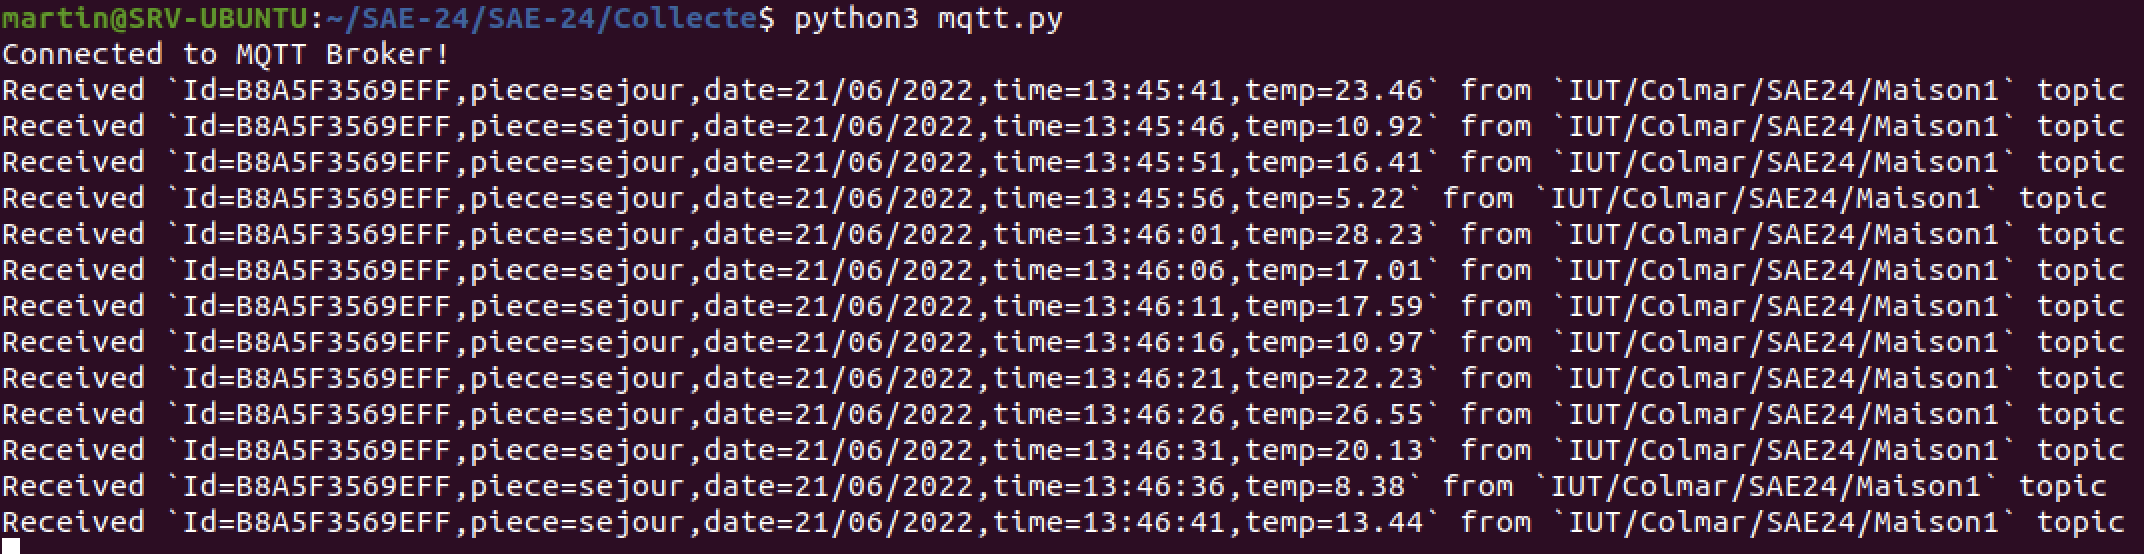
\includegraphics[width=1\textwidth]{../img/recup.png}
			\caption{Récupération des données}
			\label{fig:recup}
		\end{figure}
		Le problème est qu'il nous était demandé de récupérer un ID différent
		à chaque fois qu'une valeur de température est reçue.

	\section{Sauvegarde des valeurs dans la base de données}
		\subsection{Explications}
		L'objectif finale de cet exerice d'ensuite pouvoir sauvegarder les données dans une 
		base de données pour ensuite permettre l'affichage de ces données dans une page web.
		Pour ce faire, j'ai donc du ércrire un script qui permet premièrement la réception
		des données MQTT, puis qui les stock dans une base de données.


		\subsection{Configuration du script}
		Le script est composé de plusieurs parties. Il commence par se connecter à la base 
		de données :
		\begin{listing}[H]
			\caption{Connexion à la base de données}
			\label{lst:co}
			\begin{minted}{py}
	try:
    	db=_mysql.connect("10.37.129.3","martin","martin", "temp")
	except OperationalError:
    	db=_mysql.connect("10.37.129.3","martin","martin")
    	db.query("CREATE DATABASE martin")
    	db.query("USE martin")
			\end{minted}
		\end{listing}
		\newpage
		L'adresse IP renseigné correspond à celle de ma macbine Windows où est installé
		ma base de données :
		\begin{figure}[H]
			\centering
			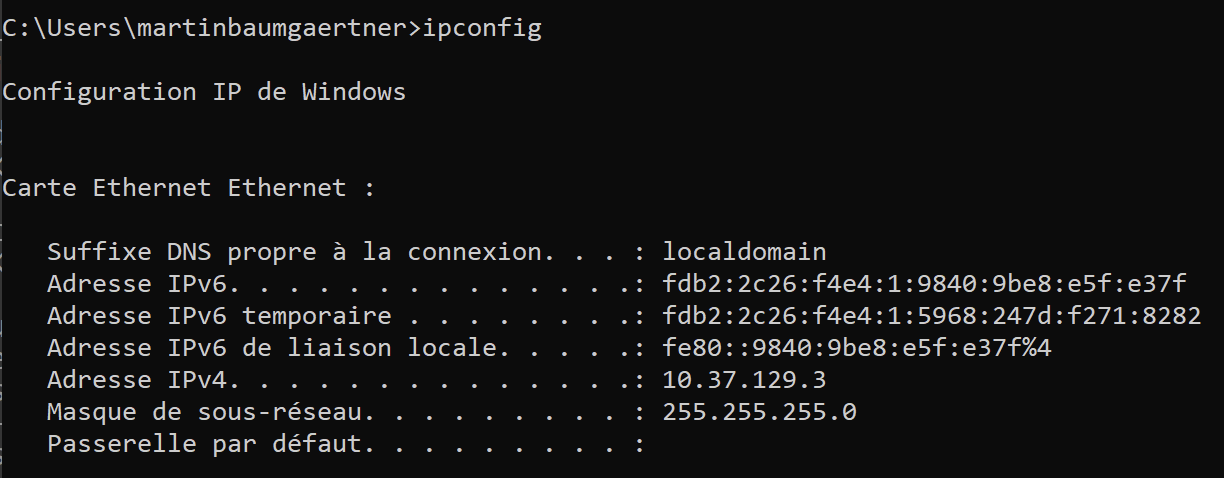
\includegraphics[width=0.6\textwidth]{../img/ip.png}
			\caption{Adresse IP de ma machine windows}
			\label{fig:ip}
		\end{figure}
	
		Puis, on défini les tables que l'on créer et les valeurs que l'on ajoute etc. :
		\begin{listing}[H]
			\caption{Création des tables}
			\label{lst:tables}
			\begin{minted}{sql}
	db.ping(True)
	db.query("""
	CREATE TABLE IF NOT EXISTS martin.sensors (
		id INT NOT NULL AUTO_INCREMENT,
		macaddr VARCHAR(12) NOT NULL,
		piece VARCHAR(50) NOT NULL,
		emplacement VARCHAR(50),
		nom VARCHAR(50),
		UNIQUE (macaddr),
		PRIMARY KEY (id))
	""")

	db.query("""
	CREATE TABLE IF NOT EXISTS martin.sensors_data (
		id INT NOT NULL AUTO_INCREMENT,
		sensor_id INT NOT NULL,
		CONSTRAINT sensorFK
			FOREIGN KEY (sensor_id)
			REFERENCES martin.sensors(id),
		datetime DATETIME NOT NULL,
		temp FLOAT NOT NULL,
		PRIMARY KEY (id))
	""")
			\end{minted}
		\end{listing}



\end{document}